\documentclass{DTETI_CP_C251}

% Penambahan Package yang akan Digunakan
\usepackage{graphicx}
\usepackage{setspace}
\usepackage{subfigure}
\usepackage{array}
\usepackage{indentfirst}
\usepackage{titlesec}
\usepackage{lipsum}
\usepackage[utf8]{inputenc}
\usepackage{multirow}
\usepackage{multicol}
\usepackage{caption}
\usepackage{longtable} 
\usepackage{algorithm}
\usepackage{algpseudocode}
% \usepackage[table,xcdraw]{xcolor}

\bibliographystyle{plain} 
\usepackage[numbers,sort&compress]{natbib}

% ------------------------------------------------------------ %
% Awal Dokumen
\begin{document}

% ------------------------------------------------------------ %
% Data Capstone
% Judul Capstone
\judul{Pembuatan \textit{Template} Laporan \textit{Capstone Project} dalam Format LaTeX}
\title{Template Design for Capstone Project Report in LaTeX Format}

% Jenis Dokumen
%% Jenis Dokumen : PERANCANGAN PRODUK DAN SPESIFIKASI

% Kode Dokumen
%% Kode Dokumen : C-251

% Nomor Dokumen (ID Kelompok Capstone)
\NoDok{C\_09}

% Nomor Revisi
\NoRev{00}

% Tanggal Penerbitan Dokumen
%% Otomatis terisi tanggal ketika file LaTeX ini di-compile

% Data Mahasiswa Capstone
%% Format : \MHS{<Nama Lengkap>}{<NIM>}{<Prodi>}{<Alamat Email>}
% Ketua Kelompok
\MHSA{Lauda Raisa}{20/xxxxxx/TK/xxxxx}
	  {Teknik Biomedis}{xxxxxx@mail.ugm.ac.id}
% Anggota 1
\MHSB{Kania}{20/xxxxxx/TK/xxxxxx}
	  {Teknik Biomedis}{xxxxxx@mail.ugm.ac.id} 
% Anggota 2
\MHSC{Muchammad Hasan Chamdany}{20/456846/TK/50670}
	  {Teknologi Informasi}{muchammadhasan@mail.ugm.ac.id}
% Anggota 3
\MHSD{Okasah}{20/xxxxxx/TK/xxxxx}
	  {Teknik Elektro}{xxxxxxx@mail.ugm.ac.id}
% Anggota 4
\MHSE{Rangga Elang}{20/xxxxxx/TK/xxxxx}
	  {Teknik Elektro}{xxxxx@mail.ugm.ac.id}
% Un-comment Line di bawah ini apabila tidak ada Anggota 4 :
% \MHSE{}{}{}{}

% Dosen Pembimbing
%% Format : {<Nama Lengkap>}{<NIP/NIU>}
\DPA{Carl Friedrich Gauss, B.Eng., M.Eng., D.Eng.}{111 1993 01 2024 01 101}

% Tempat Pelaksanaan
%% Format : {<Nama Laboratorium> \newline <Nama Departemen> \newline <Nama Fakultas>}
\Tempat{Departemen Teknik Elektro dan Teknologi Informasi \newline Fakultas Teknik}
% ------------------------------------------------------------ %
% Membuat Halaman Judul hingga Catatan Revisi Dokumen
\maketitle

% ------------------------------------------------------------ %
% Isi Laporan

% BAB 01 : Pengantar 
\chapter{\uppercase{Pengantar}}
\label{chap:Pengantar}

Di dalam bagian pengantar ini perlu dijelaskan secara ringkas mengenai topik yang akan dikerjakan, rangkuman motivasi dari pemilihan topik ini, serta ringkasan alur dan isi dari dokumen C-251 ini. Pengantar yang baik harus ditulis dengan ringkas, padat dan jelas. Sangat direkomendasikan bagian pengantar ditulis seringkas mungkin tidak melebihi 1200 kata (2 halaman).

\textcolor{black}{Topik yang dipilih dalam \textit{capstone project} ini haruslah memenuhi \underline{minimal salah satu} dari kriteria \textit{complex engineering problem} sebagai berikut:
\begin{itemize}
    \item melibatkan masalah teknis yang luas atau saling bertentangan,
    \item tidak memiliki solusi yang gamblang,
    \item solusi masalah tidak dicakup oleh standar dan kode program yang ada saat ini,
    \item melibatkan berbagai kelompok atau pemangku kepentingan,
    \item mencakup banyak bagian komponen atau sub-permasalahan,
    \item melibatkan berbagai disiplin ilmu, atau
    \item memiliki konsekuensi yang penting dalam berbagai konteks.
\end{itemize}
Penjelasan mengenai bagaimana topik yang dipilih memenuhi satu atau beberapa kriteria di atas harus diberikan pada bagian pengantar ini.
}

\section{Ujian Dokumen C-251}
\label{sec:Ujian_Dokumen_C-251}
    
    Perlu diketahui bahwa dokumen C-251 akan diuji dalam sidang yang beranggotakan komite \textit{capstone} yang akan menentukan nilai akhir mata kuliah \textit{Capstone} 1. Dokumen C-251 merupakan penutup \textit{Capstone} 1 yang merupakan suatu karya tulis yang informatif yang ditujukan untuk meyakinkan pembaca dan komite \textit{capstone} bahwa apa yang akan dilakukan dalam tugas akhir saudara adalah layak atau berharga. Selain itu, \textit{Capstone} 1 berusaha memberikan jaminan bahwa apa yang akan dilakukan bisa diimplementasikan dalam waktu yang masuk akal (biasanya tiga sampai enam bulan).

\section{Informasi Singkat Mengenai \textit{Template} Dokumen C-251}
\label{sec:Informasi_Singkat_Mengenai_Template_Dokumen_C-251}

    \subsection{Susunan \textit{Directory}}
    \label{subsec:Susunan_Directory}
    
        \textit{Template} dokumen C-251 ini tersusun oleh beberapa \textit{directory} yang digunakan untuk memudahkan organisasi \textit{file-file} yang menjadi penyusun dokumen C-251 ini. Pada tingkat ke-1, terdapat 2 (dua) \textit{directory}/\textit{folder} seperti yang ditunjukkan oleh Tabel \ref{tab:Ch01_Directory_Level_1}.
        
        \begin{longtable}{|C{0.7cm}|C{1.8cm}|L{12.5cm}|}
            \caption{Susunan \textit{Directory} Tingkat Ke-1}
            \label{tab:Ch01_Directory_Level_1}
            \vspace{-0.75em}\\
            \hline
                \textbf{No}                                     &
                \textbf{\textit{Directory}}                     &
                \multicolumn{1}{C{12.5cm}|}{\textbf{Keterangan}} \\
            \hline
                1   &
                fig &
                Berisi \textit{file-file} gambar yang akan digunakan di dalam dokumen C-251. \\
            \hline
                2       &
                thesis  &
                Berisi \textit{directory-directory} yang di dalamnya terdapat \textit{file-file} penyusun dokumen C-251.\\
            \hline
        \end{longtable}
        
        \noindent Kemudian di dalam \textit{directory} "thesis", terdapat beberapa \textit{directory} penyusun seperti yang ditunjukkan oleh Tabel \ref{tab:Ch01_Directory_Level_2_fig}.
        
        \begin{longtable}{|C{0.7cm}|C{2.8cm}|L{11.5cm}|}
            \caption{Susunan \textit{Directory} Tingkat Ke-2 di dalam \textit{Directory} "thesis"}
            \label{tab:Ch01_Directory_Level_2_fig}
            \vspace{-0.75em}\\
            \hline
                \textbf{No}                                         &
                \textbf{\textit{Directory}}                         &
                \multicolumn{1}{C{11.5cm}|}{\textbf{Keterangan}}    \\
            \hline
                1   &
                Catatan\_Revisi &
                Berisi \textit{file-file} yang digunakan untuk mendeskripsikan catatan-catatan dari revisi yang telah dilakukan. \\
            \hline
                2       &
                Isi\_Laporan  &
                Berisi \textit{file-file} yang digunakan untuk menuliskan isi dari laporan/dokumen C-251 ini.\\
            \hline
                3       &
                Main  &
                Berisi \textit{file} untuk menuliskan intisari dokumen ("Intisari.tex"), data-data mengenai dokumen C-251 ("Data\_Capstone.tex"), dan daftar pustaka ("Referensi.tex"). Selain itu berisi juga \textit{file} yang mengatur formatting dari dokumen C-251 ini ("DTETI\_CP\_C251.cls") beserta file utama yang menggabungkan semua komponen penyusun dokumen C-251 ini ("main.tex").\\
            \hline
        \end{longtable}
    
    \subsection{Pengisian Data Mengenai Dokumen C-251}
    \label{subsec:Pengisian_Data_MEngenai_Dokumen_C-251}
    
        Hal pertama yang harus Anda lakukan ketika menggunakan \textit{template} \LaTeX ini adalah mengisi data-data dasar mengenai dokumen C-251 ini. Pengisian data-data tersebut dilakukan pada \textit{file} "Data\_Capstone.tex" yang berada di dalam \textit{directory} "thesis/Main/". Data-data yang perlu Anda isikan ditunjukkan oleh Tabel \ref{tab:Ch01_Data_Dokumen_C-251}.
        
        \begin{longtable}{|C{0.7cm}|C{1.8cm}|L{12.5cm}|}
            \caption{Data-Data Dokumen C-251}
            \label{tab:Ch01_Data_Dokumen_C-251}
            \vspace{-0.75em}\\
            \hline
                \textbf{No}                                         &
                \textbf{Data}                                       &
                \multicolumn{1}{C{12.5cm}|}{\textbf{Keterangan}}    \\
            \hline
                1   &
                judul &
                Usulan judul \textit{capstone} dalam Bahasa Indonesia. \\
            \hline
                2   &
                title &
                Usulan judul \textit{capstone} dalam Bahasa Inggris. \\
            \hline
                3   &
                NoDok &
                Kode tim/kelompok \textit{capstone}. \\
            \hline
                4   &
                NoRev &
                Nomor revisi dokumen. \\
            \hline
                5   &
                MHSA &
                Nama lengkap, NIM, program studi dan alamat \textit{email} ketua kelompok. \\
            \hline
                6   &
                MHSB &
                Nama lengkap, NIM, program studi dan alamat \textit{email} anggota 1. \\
            \hline
                7   &
                MHSC &
                Nama lengkap, NIM, program studi dan alamat \textit{email} anggota 2. \\
            \hline
                8   &
                MHSD &
                Nama lengkap, NIM, program studi dan alamat \textit{email} anggota 3. \\
            \hline
                9   &
                MHSE &
                Nama lengkap, NIM, program studi dan alamat \textit{email} anggota 4. \\
            \hline
                10   &
                DPA &
                Nama lengkap dan NIP/NIU dari Dosen Pembimbing. \\
            \hline
                11   &
                Tempat &
                Tempat pelaksanaan \textit{capstone}. \\
            \hline
        \end{longtable}
        
        \noindent Pastikan Anda mengisi data-data tersebut dengan benar sehingga informasi yang tertampil pada halaman judul dan halaman pengesahan merupakan informasi yang benar.
    
    \subsection{Melampirkan Bukti Bebas Plagiasi}
    \label{subsec:Melampirkan_Bukti_Bebas_Plagiasi}
    
        Ketika mengumpulkan dokumen C-251 ini, Anda \uline{wajib} untuk melampirkan bukti bahwa dokumen C-251 yang Anda susun telah bebas dari plagiasi. Yang perlu Anda lakukan adalah melampirkan halaman utama dari \textit{similarity report} yang telah Anda terima seperti yang terlihat pada contoh. Berikut ini adalah langkah-langkah yang perlu Anda lakukan dalam proses pelampiran bukti bebas plagiasi.
        
        \begin{enumerate}
            \item Anda mengirimkan dokumen C-251 Anda yang telah siap untuk dilakukan pengecekan plagiasi. Mekanisme detail mengenai proses pengecekan plagiasi ini akan diumumkan di kemudian hari.
            \item Anda akan mendapatkan \textit{file} \textit{similarity report} dalam bentuk PDF yang menunjukkan seberapa besar kemiripan antara konten dokumen C-251 yang Anda susun dengan sumber-sumber yang ada di internet.
            \item Apabila hasil pengecekan plagiasi tersebut telah memenuhi kriteria yang diizinkan, maka Anda perlu mengambil halaman utama dari file \textit{similarity report} tersebut yang menunjukkan \textit{Originality Report} dari dokumen C-251 Anda. Proses pengambilan halaman ini dapat Anda lakukan melalui laman-laman \textit{online}, misalnya adalah laman "https://smallpdf.com/split-pdf".
            \item Gantilah nama \textit{file} tersebut menjadi "Bukti\_Bebas\_Plagiasi.pdf", kemudian letakkan \textit{file} tersebut di dalam \textit{directory} "fig". Mohon diperhatikan penamaan \textit{file} bukti bebas plagiasi tersebut. Apabila penamaan \textit{file} tersebut tidak sesuai dengan ketentuan, maka akan muncul pesan \textit{error} ketika Anda melakukan kompilasi (meng-\textit{compile}).
        \end{enumerate}
        
    \subsection{Menuliskan Catatan Revisi Dokumen}
    \label{subsec:Menuliskan_Catatan_Revisi_Dokumen}
    
    Catatan revisi dokumen di dalam dokumen C-251 ini ditujukan untuk mencatat revisi-revisi yang dilakukan selama proses penulisan dokumen C-251 ini. Proses revisi dokumen tersebut muncul biasanya dilakukan ketika adanya permintaan perbaikan dokumen dari dosen pembimbing, maupun dari dosen penguji ketika ujian dokumen C-251. Poin-poin revisi yang dilakukan tersebut wajib didokumentasikan di dalam bab catatan revisi dokumen ini.
    
    Dalam \textit{template} dokumen C-251 ini, penulisan catatan revisi dokumen dilakukan dengan cara mengisi \textit{file-file} di dalam \textit{directory} "Catatan\_Revisi". Di dalam \textit{directory} tersebut telah disediakan total 10 (sepuluh) \textit{file} yang digunakan untuk menuliskan catatan revisi tersebut. Nama dari \textit{file-file} tersebut dimulai dari "Revisi\_00.tex" hingga "Revisi\_09.tex". Masing-masing \textit{file} tersebut diperuntukkan untuk pencatatan 1 (satu) proses revisi dokumen. 
    
    \textit{File} "Revisi\_00.tex" wajib diisi untuk memberikan keterangan singkat mengenai versi awal dari dokumen C-251 ini. Untuk revisi ke-1 dan selanjutnya, catatan revisi tersebut dapat dituliskan pada \textit{file} "Revisi\_01.tex", "Revisi\_02.tex", dst. Perlu diperhatikan bahwa banyaknya catatan revisi yang akan ditampilkan ditentukan oleh nilai "NoRev" yang diisikan pada \textit{file} "Data\_Capstone.tex". Apabila nilai "NoRev" adalah "1" atau "01", maka hanya konten di dalam \textit{file} "Revisi\_00.tex" dan "Revisi\_01.tex" saja yang akan ditampilkan. Sedangkan apabila nilai "NoRev" adalah "3" atau "03", maka hanya konten di dalam \textit{file} "Revisi\_00.tex", "Revisi\_01.tex", "Revisi\_02.tex" dan "Revisi\_03.tex" yang akan ditampilkan. Oleh karena itu, perlu dilakukan sinkronisasi antara nilai "NoRev" dengan catatan revisi yang dituliskan di dalam \textit{file} "Revisi\_xx.tex".
    
\section{Contoh Penulisan Dokumen Menggunakan \LaTeX}
\label{sec:Contoh_Penulisan_Dokumen_Menggunakan_LaTeX}

    \subsection{Persamaan Matematis}
    \label{subsec:pers_mat}
    
        Persamaan dapat ditulis dengan berbagai cara. Untuk persamaan yang sederhana dapat menggunakan penulisan berikut.
        
        \begin{equation}
            \label{eqn:short}
            a+b=\gamma
        \end{equation}
        
        \noindent Sedangkan persamaan yang cukup panjang dapat ditulis dalam beberapa baris seperti berikut.
        \begin{equation}
            \label{eqn:long1}
            \begin{split}
                1+2+3+4+8x+7 & =1+2+3+4+4x+35 \\
                & \Rightarrow x=7
            \end{split}
        \end{equation}
        
        \noindent atau sebagai berikut.
        \begin{align}
            \label{eqn:long2}
            (x+y)^3&=(x+y)(x+y)^2\\
                   &=(x+y)(x^2+2xy+y^2)\\
                   &=x^3+3x^2y+3xy^3+x^3.
        \end{align}
        
        Jika Anda ingin hanya menggunakan satu nomor persamaan pada persamaan yang \textit{multi-line}, maka dapat dilakukan dengan
        \begin{align}
            \label{eqn:long3}
            \begin{split}
                 (x+y)^3&=(x+y)(x+y)^2\\
                       &=(x+y)(x^2+2xy+y^2)\\
                       &=x^3+3x^2y+3xy^3+x^3.
            \end{split}
        \end{align}
        
        \noindent Ketika persamaan diacu pada teks, maka dapat dilakukan dengan cara  kata "Persamaan~(\ref{eqn:short})".
    
    \subsection{Gambar dan Tabel}
    \label{subsec:gmbr_tab}
        
        Posisi gambar atau table harus berada pada bagian atas atau bawah pada tiap halaman. Judul gambar berada di bawah gambar, sedangkan judul tabel berada di atas table. Gunakan kata "Gambar~\ref{fig:example1}" atau "Tabel~\ref{tab:example1}" untuk mengacu gambar atau tabel dalam naskah.
        
        %%=============================
        \begin{figure}[!ht]
            \centering
            
\includegraphics{fig1.png}
            \caption{Contoh Gambar}
            \label{fig:example1}
        \end{figure}
    
        %%========================
        \begin{longtable}{|c|c|c|c|c|}
            \caption{Contoh Tabel}
            \label{tab:example1}
            \vspace{-0.75em}\\
            \hline
            \textbf{No} & \textbf{Spesifikasi}  & \textbf{Satuan} & \textbf{Standar} & \textbf{Keterangan} \\ \hline
            1           & Tegangan Masukan      & Volt (V)        & 95 sampai 220 V  & Lihat Penjelasan A  \\ \hline
            2           & Tegangan Keluaran     & Volt (V)        & 20 V $\pm$ 0,2\% & Lihat Penjelasan B  \\ \hline
            3           & Interferensi Magnetis & Watt (W)        & Maksimal 0,1 W   & Lihat Penjelasan C  \\ \hline
            4           & SNR                   & Decibel (dB)    & Minimum 80 dB    & Lihat Penjelasan D  \\ \hline
            5           & dan seterusnya        &                 &                  &                     \\ \hline
        \end{longtable}
        
        Dalam penulisan tabel, sangat disarankan untuk menggunakan \textit{environment} "longtable" seperti Tabel \ref{tab:example1}. Penggunaan "longtable" ini bertujuan agar tabel dapat terpisahkan ke dalam beberapa halaman yang berbeda apabila memang ukuran tabel tersebut terlalu panjang. Hal ini tidak dapat diakomodasi oleh \textit{environment} "table" yang standar.
        
        Sama seperti ketika menggunakan MS Word, posisi teks di dalam tabel dapat diatur sesuai dengan keinginan. Hal ini dilakukan dengan memilih opsi "l", "c" atau "r" yang diletakkan setelah perintah untuk memulai \textit{environtment} "longtable". Contoh penggunana masing-masing opsi \textit{alignment} ini ditunjukkan pada Tabel \ref{tab:alignment_01}.
        
        \begin{longtable}{|c|l|c|r|}
            \caption{Contoh Penggunaan \textit{Alignment} dengan Lebar Kolom yang Otomatis}
            \label{tab:alignment_01}
            \vspace{-0.75em}\\
            \hline
                \textbf{Opsi} & l & c & r    \\
            \hline
                \textbf{Posisi Horizontal} & Kiri & Tengah & Kanan \\
            \hline
                \textbf{Posisi Vertikal} & Tengah & Tengah & Tengah \\
            \hline
        \end{longtable}
        
        Salah satu fitur dari ketiga opsi \textit{alignment} tersebut adalah ukuran lebar kolom tabel akan secara otomatis menyesuaikan dengan panjang teks. Akan tetapi, terkadang fitur ini menjadi kurang baik karena lebar tabel secara keseluruhan dapat melewati margin yang telah ditentukan. Oleh karena itu, dalam \textit{template} \LaTeX ini disediakan pula opsi \textit{alignment} lainnya seperti yang ditunjukkan oleh Tabel \ref{tab:alignment_02}.
        
        \begin{longtable}{|C{3.2cm}|L{2cm}|C{2cm}|R{2cm}|}
            \caption{Contoh Penggunaan \textit{Alignment} dengan Lebar Kolom Tertentu}
            \label{tab:alignment_02}
            \vspace{-0.75em}\\
            \hline
                \textbf{Opsi} & L & C & R    \\
            \hline
                \textbf{Posisi Horizontal} & Kiri & Tengah & Kanan \\
            \hline
                \textbf{Posisi Vertikal} & Tengah & Tengah & Tengah \\
            \hline
        \end{longtable}
        
        \noindent Dengan menggunakan opsi-opsi tersebut, maka dapat dimungkinkan untuk membuat sebuah tabel dengan ukuran lebar kolom yang seragam.

    \subsection{Sitasi}
    \label{subsec:sitasi}
    
        Gunakanlah sitasi berupa angka dengan menggunakan \textit{brackets} seperti berikut~\cite{edwards_sliding_1998}. Tanda baca seperti titik (\textit{full stop}) mengikuti \textit{brackets} \cite{b1}. Gunakalanlah sitasi dengan mengacu pada nomornya saja seperti pada  \cite{b2}---jangan gunakan ``Ref. \cite{b3}'' atau ``referensi \cite{b3}'' kecuali pada awal kalimat: ``Referensi \cite{b3} menggunakan $\ldots$''.
        
        Jika melakukan sitasi pada lebih dari satu sumber pada saat yang bersamaan, maka gunakanlah \cite{edwards_sliding_1998, b1} atau \cite{edwards_sliding_1998, b1, b2, b3}.
    
       % Tuliskan semua nama \textit{author} kecuali jika jumlah authornya lebih dari enam \textit{author} atau lebih di mana anda bisa menggunakan: . 
       
       
    \subsection{Algoritme}
    \label{subsec:algo}
    
    Anda dapat menulis algortime seperti pada contoh "Algoritme~\ref{algo:algo1}". 
    \begin{algorithm}
    	\caption{PPO} 
    	\label{algo:algo1}
    	\begin{algorithmic}[1]
    		\For {$iteration=1,2,\ldots$}
    			\For {$actor=1,2,\ldots,N$}
    				\State Run policy $\pi_{\theta_{old}}$ in environment for $T$ time steps
    				\State Compute advantage estimates $\hat{A}_{1},\ldots,\hat{A}_{T}$
    			\EndFor
    			\State Optimize surrogate $L$ wrt. $\theta$, with $K$ epochs and minibatch size $M\leq NT$
    			\State $\theta_{old}\leftarrow\theta$
    		\EndFor
    	\end{algorithmic} 
    \end{algorithm}
    


% BAB 02 : Dasar Teori Pendukung 
\chapter{\uppercase{Dasar Teori Pendukung}}
\label{chap:Dasar_Teori_Pendukung}
Uraikan semua dasar teori pendukung tugas akhir ini dengan terstruktur dan sistematis. Terstruktur dan sistematis artinya semua teori yang diperlukan dapat disajikan dengan urutan yang baik sehingga tidak terjadi perulangan di belakang. Misalnya teori dan semua variabel setelah dideklarasikan, maka akan dipakai seterusnya tanpa mengulangi definisi teori dan variabel tersebut kecuali jika secara spesifik diperlukan. 

Walaupun berupa dasar teori, tim \textit{capstone} \uline{harus menuliskannya sendiri} dan \textbf{\uline{dilarang keras} \uline{untuk melakukan \textit{copy and paste}}} serta \uline{wajib bebas dari plagiarisme}. Menyunting diperbolehkan selama memenuhi kriteria akademis dengan memberikan referensi yang tepat. Mahasiswa diharapkan untuk bisa belajar tentang etika akademik yang berkaitan dengan cara menyunting untuk menghindari praktek plagiarisme kepada dosen pembimbing \textit{capstone} masing-masing.

Sebagai contoh, berikut ini adalah dasar teori yang menjelaskan mengenai interpretasi geometris dari konsep \textit{eigenvalue} dan \textit{eigenvector}.

\section{Intepretasi Geometris dari \textit{Eigenvalues} dan \textit{Eigenvectors}}
\label{sec:Interpretasi_Geometris_Eigenvalue_Eigenvector}

    Dalam ilmu Aljabar Linear, ketika sebuah matriks $A$ dikalikan dengan sebuah vektor $v$, makna dari proses perkalian tersebut adalah matriks $A$ tersebut mentransformasikan vektor $v$ menjadi sebuah vektor baru $w = T(v) = Av$. Ide dari transformasi $T(v)$ tersebut sama dengan ide dari fungsi $y = f(x)$, yang mana akan menghasilkan sebuah nilai baru $y$ ketika kita memasukkan sebuah nilai tertentu $x$ ke dalam fungsi tersebut. 
    
    \begin{figure}[h!]
        \centering
        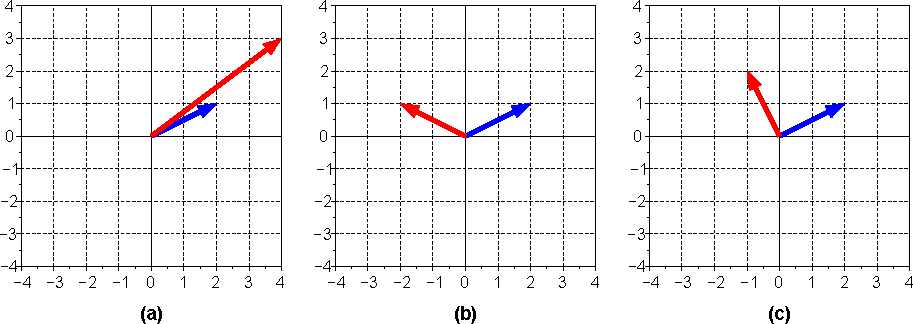
\includegraphics[scale=1.0]{Ch02_Vector_Transformation.pdf}
        \caption{Efek dari 3 Matriks Transformasi yang Berbeda terhadap Vektor $v$ (Biru)}
        \label{fig:Ch02_Vector_Transformation}
    \end{figure}
        
    Macam dari matriks transformasi $A$ tersebut sangatlah banyak, antara lain :
    \begin{equation}
    	\label{eqn:Ch02_Transformation_Matrix}
    	\begin{split}
    		A_1 =
    		\begin{bmatrix}
    			2 & 0 \\ 0 & 3
    		\end{bmatrix}
    		\quad \text{;} \quad
    		A_2 =
    		\begin{bmatrix}
    			-1 & 0 \\ 0 & 1
    		\end{bmatrix}
    		\quad \text{;} \quad
    		A_3 =
    		\begin{bmatrix}
    			0 & -1 \\ 1 & 0
    		\end{bmatrix}
    	\end{split}
    \end{equation}
    Representasi grafis dari masing-masing matriks transformasi tersebut dapat dilihat pada Gambar \ref{fig:Ch02_Vector_Transformation}. Seperti yang ditunjukkan pada Gambar \ref{fig:Ch02_Vector_Transformation}(a), matriks transformasi $A_1$ merupakan sebuah matriks \textit{scaling}, yang mengubah panjang komponen sumbu $x$ dari vektor $v$ menjadi 2 kalinya, dan panjang komponen sumbu $y$ dari vektor $v$ menjadi 3 kalinya. Sedangkan untuk matriks transformasi $A_2$, matriks ini digunakan untuk mencerminkan vektor $v$ terhadap sumbu $y$ seperti yang ditunjukkan oleh Gambar \ref{fig:Ch02_Vector_Transformation}(b). Terakhir, untuk matriks transformasi $A_3$ merupakan matriks rotasi, yang merotasi vektor $v$ sejauh $90^o$ dengan arah berlawanan dengan arah jarum jam seperti yang ditunjukkan oleh Gambar \ref{fig:Ch02_Vector_Transformation}(c).
    

% BAB 03 : Analisis Studi Pustaka Kunci 
\chapter{\uppercase{Analisis Studi Pustaka Kunci}}
\label{chap:Analisis_Studi_Pustaka_Kunci}


Salah satu kemampuan yang harus dimiliki oleh seorang Sarjana Teknik adalah kemampuan menganalisis sumber-sumber pustaka. Oleh karena itu, di dalam dokuman C-251 ini, mahasiswa perlu melakukan studi pustaka dan menuliskannya sampai kepada level kedalaman dan detail yang memadai. Sebelum melakukan analisis pustaka, uraikan lagi apa saja permasalahan yang ingin Anda selesaikan di dalam \textit{capstone} ini. Dari permasalahan tersebut, carilah literatur yang sudah pernah membahas dan menyelesaikan masalah yang sama, dan pilihkan pustaka kunci yang akan Anda adopsi untuk membantu menyelesaikan Anda. 

\textcolor{black}{Di bagian ini, tunjukkan bahwa masalah yang dipilih memiliki solusi terbuka (\textit{open-ended solution}), yaitu memiliki minimal 3 solusi potensial yang ada di literatur.}

\textcolor{black}{Mahasiswa juga dituntut untuk mengevaluasi solusi-solusi yang mungkin berdasarkan proses dan standar keteknikan. \textbf{Mahasiswa tidak diperkenankan hanya menyajikan solusi yang didapat di literatur. Mahasiswa perlu menunjukkan keunggulan dan kelemahan setiap solusi tersebut}. Untuk mencapai poin tersebut, di Bab ini, mahasiswa harus mengacu pada minimal 10 buah referensi dalam mengevaluasi solusi-solusi potensial dari permasalahan yang dipilih. Literatur sebaiknya diambilkan dari sumber ilmiah seperti jurnal, standard, ataupun \textit{technical report}
}

Buatlah analisis yang mendalam dan jika perlu disimulasikan metodenya untuk menyelesaikan permasalahan Anda. Uraikan secara ringkas sumber-sumber yang membahas berbagai kerangka teori dan metode-metode yang mungkin untuk digunakan secara sistematis. Gunakan \textit{heading} untuk menguraikan metode yang ada.


\section{Metode 1}
\label{sec:Metode_01}

    \lipsum[1-3]

\section{Metode 2}
\label{sec:Metode_02}

    \lipsum[4-6]
    
    \subsection{Sub-Metode 2}
    \label{subsec:Sub-Metode_02}
    
    \lipsum[7-9]

\section{Metode 3}
\label{sec:Metode_03}

    \lipsum[10-12]
    
    \subsection{Sub-Metode 3A}
    \label{subsec:Sub-Metode_03A}
    
    \lipsum[13-15]
    
    \subsection{Sub-Metode 3B}
    \label{subsec:Sub-Metode_03B}
    
    \lipsum[15-18]

% BAB 04 : Pemodelan Permasalahan 
\chapter{\uppercase{Pemodelan Permasalahan}}
\label{chap:Pemodelan_Permasalahan}
Salah satu tujuan pendidikan insinyur adalah kemampuan membuat lulusan untuk bisa secara luwes menggunakan sains natural (IPA) dan Matematika untuk membantu menyelesaikan permasalahan nyata di industri dan di masyarakat. 
Untuk membantu menyelesaikan masalah secara sistematis, sangat disarankan mahasiswa mampu memodelkan permasalahan ke dalam persamaan matematika. Jika tidak dimungkinkan secara matematis, maka diperbolehkan pemodelan dengan cara yang lain misalnya secara heuristik, secara statistik, secara empiris, dan lain-lain.

Sebagai gambaran tim mahasiswa, di akhir dokumen ini mahasiswa perlu mengusulkan perancangan mendetail. Sehingga pemodelan di sini sangat menentukan level akurasi dan kualitas desain yang diusulkan. Sebagai contoh jika mahasiswa akan membuat desain kendali maka di bagian pemodelan mahasiswa memodelkan \textit{plant} ke dalam \textit{state-space} atau fungsi alih (\textit{transfer function}) seperti yang ditunjukkan pada (\ref{eqn:Ch04_Transfer_Function_Motor_DC}) sebagai berikut.

\begin{equation}
    \label{eqn:Ch04_Transfer_Function_Motor_DC}
    H(s) = \dfrac{K_t}{\left( sL + R \right) \left( sJ + b \right) + K_t K_i}
\end{equation}

Jika mahasiswa ingin mendesain sistem sensor, mahasiswa perlu memodelkan sifat-sifat fisika dari medium dan besaran yang akan diukur dan sebagainya, Jika ingin membuat sistem elektronis, misalnya lampu lalu lintas cerdas, mahasiswa perlu memodelkan arus pergerakan kendaraan di persimpangan jalan, dan lain-lain.

Pada sub-bab perancangan detail nanti mahasiswa akan menganalisis lebih lanjut model plant tersebut ke dalam analisa kestabilan dengan Aljabar Linear, Routh-Hutwitz, Root-Locus, kurva Bode atau Nyquist dan lain-lain untuk bisa mengenal lebih mendalam tentang \textit{plant} sehingga bisa mendesain pengendali yang tepat, membuat algoritme pengendalian, menentukan \textit{hardware} atau \textit{software}, melakukan \textit{coding} atau pemrograman, dan menanamkannya pada \textit{microcontroller} atau komputer atau perangkat yang lain. Untuk mendesain lampu lalu lintas cerdas solusi macet, mahasiswa akan menggunakan model ini untuk menentukan \textit{timing} yang tepat dan paling optimal, dan lain sebagainya. 



% BAB 05 : Pemilihan dan Pengembangan Metode 
\chapter{\uppercase{Pemilihan dan Pengembangan Metode}}
\label{chap:Pemilihan_dan_Pengembangan_Metode}
\textcolor{black}{Sebagaimana telah disinggung di \ref{chap:Dasar_Teori_Pendukung}, mahasiswa dituntut untuk mengevaluasi solusi-solusi yang mungkin berdasarkan proses dan standar keteknikan. Untuk mencapai poin tersebut, di Bab ini, mahasiswa harus memilih solusi terbaik untuk permasalahan spesifik yang telah dipilih.} Setelah dideskripsikan kekurangan dan kelebihan metode, tim akan memilih metode yang paling tepat disertai pengembangan metode tersebut. Jika dari semua metode yang ada tidak menghasilkan solusi yang konkret, tim bisa membuat metode sendiri. Dalam hal ini, proyek \textit{capstone} ini akan menjalankan mode penelitian sehingga tidak diwajibkan untuk menghasilkan luaran tertentu. Walaupun begitu adanya luaran seperti tertulis pada lembar luaran sangat disarankan. 



% BAB 06 : Luaran dan Spesifikasi yang Diusulkan 
\chapter{\uppercase{Luaran dan Spesifikasi yang Diusulkan}}
\label{chap:Luaran_dan_Spesifikasi_yang_Diusulkan}
Pada bagian ini, mahasiswa menjelaskan luaran (\textit{output}) apa yang dijanjikan di akhir periode capstone. Bagian ini harus disinkronkan dengan lembar luaran pada awal dokumen ini. Ada berbagai jenis luaran yang harus dihasilkan minimal satu oleh mahasiswa seperti disebutkan pada lembar luaran.

\textcolor{black}{Sebagaimana telah disinggung di \ref{chap:Dasar_Teori_Pendukung}, mahasiswa juga dituntut untuk mengevaluasi solusi-solusi yang mungkin berdasarkan proses dan standar keteknikan. Untuk mencapai poin tersebut, di Bab ini, mahasiswa harus menentukan kebutuhan, spesifikasi, atau standar dari solusi yang diusulkan di bagian \ref{sec:Spesifikasi_Luaran}. Selain itu, \textbf{mahasiswa harus menentukan kriteria sukses/keberhasilan dari solusi yang dipilih}. Kriteria sukses biasanya didefinisikan jika semua spesifikasi luaran sudah terpenuhi} 

\section{Luaran yang Dijanjikan}
\label{sec:Luaran_yang_Dijanjikan}

    Pada bagian ini, mahasiswa menjelaskan luaran (\textit{output}) apa yang dijanjikan di akhir periode \textit{capstone}. Bagian ini harus disinkronkan dengan lembar luaran pada awal dokumen ini. Ada berbagai jenis luaran yang harus dihasilkan minimal satu oleh mahasiswa seperti disebutkan pada lembar luaran seperti yang dapat dituliskan pada Tabel \ref{tab:Ch06_Contoh_Luaran}.
    
    \begin{longtable}{|L{7.5cm}|L{7.5cm}|}
        \caption{Contoh Luaran} 
        \label{tab:Ch06_Contoh_Luaran}
        \vspace{-0.75em}\\        
        \hline
        \multicolumn{1}{|c|}{\textbf{Jenis Luaran}}                                                                     & \multicolumn{1}{c|}{\textbf{Contoh}}                                                                                \\ \hline
        
        \textit{Hardware} Digital (fisik)                                                                                        & Alat pendeteksi asap berbasis mikroprosesor                                                                         \\ \hline
        
        \textit{Hardware} Analog (fisik)                                                                                         & Alat penghasil frekuensi 1 THz menggunakan rangkaian RLC                                                            \\ \hline
        
        \textit{Firmware}/SW di Mikroprosesor/\textit{Development Board}                                                                  & Alat untuk memonitor asap berbasis komputer                                                                         \\ \hline
        
        \textit{Software} di PC                                                                                                  & Software untuk mendeteksi asap berbasis Python                                                                      \\ \hline
        
        Sistem Informasi                                                                                                & Sistem informasi \textit{capstone} mahasiswa, Sistem informasi manajemen kebakaran                                           \\ \hline
        Simulasi Lengkap                                                                                                & Simulasi dan mitigasi black-out di sistem transmisi 500~kV      \\ \hline
        
        Prototipe/miniatur \textit{hardware}/\textit{software}/sistem                                                                     & Prototipe lampu lalu lintas cerdas perempatan MM-UGM                                                                \\ \hline
        
        Teorema/Teori Baru                                                                                              & Teori kestabilan sistem tenaga terbarukan dengan beban negatif resistif                                             \\ \hline
        
        Kebaruan/\textit{novelty} yang lain/perbaikan metode (apabila berupa \textit{capstone} penelitian)                                & Perbaikan faktor daya dengan metode Alpha, Pencarian jarak terpendek pada sensor asap                               \\ \hline
        
        Dokumen (Kebijakan, SOP, Lingkungan, Ekonomi, dll)                                                              & SOP teknis perencanaan sistem proteksi, Dokumentasi \textit{black-out} dan analisisnya, Dokumen usulan investasi energi, dll \\ \hline
        
        \begin{tabular}[C{7.5cm}]{@{}L{7.5cm}@{}}Lain-lain (sebutkan)\\ Contoh : Simulasi parsial (dengan \textit{software} jadi)\end{tabular} & Contoh : Simulasi trafo dengan Fluent                                                                            \\ \hline
    \end{longtable}
    
\section{Spesifikasi Luaran}
\label{sec:Spesifikasi_Luaran}

    Pada bagian ini, target performa yang akan dicapai berdasarkan fungsionalitas sebagai syarat keberhasilan kinerja produk harus dicantumkan (misal : modul kontroller dapat mengurangi \textit{overshoot} hingga dibawah 1\% atau akurasi produk di bawah 0.01\%). Yang perlu ditekankan disini mahasiswa harus menggunakan standar-standar keteknikan (besaran dan satuan, \textit{policy}/aturan, dan lain-lain) yang disepakati oleh organisasi keteknikan misalnya IEEE, PUIL, ACM dan lain-lain. Contoh spesifikasi luaran yang baik adalah seperti pada Tabel \ref{tab:Ch06_Contoh_Spesifikasi_Luaran}.
    
    \begin{longtable}{|c|c|c|c|c|}
        \caption{Contoh Spesifikasi Luaran} 
        \label{tab:Ch06_Contoh_Spesifikasi_Luaran}
        \vspace{-0.75em}\\
        \hline
        \textbf{No} & \textbf{Spesifikasi}  & \textbf{Satuan} & \textbf{Standar} & \textbf{Keterangan} \\ \hline
        1           & Tegangan Masukan      & Volt (V)        & 95 sampai 220 V  & Lihat Penjelasan A  \\ \hline
        2           & Tegangan Keluaran     & Volt (V)        & 20 V $\pm$ 0,2\% & Lihat Penjelasan B  \\ \hline
        3           & Interferensi Magnetis & Watt (W)        & Maksimal 0,1 W   & Lihat Penjelasan C  \\ \hline
        4           & SNR                   & Decibel (dB)    & Minimum 80 dB    & Lihat Penjelasan D  \\ \hline
        5           & dan seterusnya        &                 &                  &                     \\ \hline
    \end{longtable}
    
  

% BAB 07 : Batasan Permasalahan 
\chapter{\uppercase{Batasan Permasalahan}}
\label{chap:Batasan_Permasalahan}
Pada bagian ini peserta \textit{capstone} menguraikan lebih lanjut spesifikasi dari rancangan produk di atas. Spesifikasi yang dimaksud di sini adalah spesifikasi yang bersifat fungsional. Tim juga harus mendefinisikan batasan-batasan permasalahan secara lebih terperinci dan konkret. Batasan-batasan ini diperlukan untuk membuat sistem yang dirancang bisa diimplementasikan secara masuk akal dalam jangka waktu, kesediaan sarana dan prasarana, jumlah sumber daya manusia (SDM), biaya yang terbatas, dan lain-lain. 

Pada bidang TI, peserta \textit{capstone} dapat menjelaskan fasilitas atau fitur apa saja yang disediakan oleh sistem yang dirancang secara lebih detail. Sebagai contoh, sistem informasi keuangan dapat dispesifikasikan untuk memiliki kemampuan untuk melakukan perhitungan biaya atau gaji (\textit{payroll}) berserta laporan (\textit{reporting}). Pada kasus ini, peserta wajib menyebutkan secara detail jenis pelaporan yang ada. Kemudian, perlu juga dijelaskan bagaimana perhitungan tersebut dilakukan, serta \textit{user} apa saja yang dikehendaki terlibat dalam sistem yang dirancang. Di samping itu, peserta wajib mencantumkan apa saja keterbatasan sistem yang dirancang, misalnya fitur apa saja yang tidak dapat atau tidak akan dilakukan atau tidak disediakan pada produk yang akan dikembangkan. 

Pada bidang TE yang menghasilkan perangkat keras, dapat dijelaskan mengenai fitur fungsional dan karakteristik dari perangkat keras tersebut. Sebagai contoh, misalkan sebuah rancangan robot diharapkan dapat digunakan untuk membantu orang tua yang memiliki keterbatasan. Dalam memenuhi tugas tersebut, robot dapat dispesifikasikan memiliki kriteria tertentu, misalkan, stabil pada kondisi medan yang homogen maupun heterogen (lapangan rumput, aspal, con-block). Selain, itu robot dapat dispesifikasikan memiliki bentuk yang kokoh dan rapi, pengkabelan (\textit{wiring}) tidak berantakan, tertutup dan aman. Perlu disebutkan juga keterbatasan robot tersebut, misalnya hanya membahas robot beroda dan tidak bisa bergerak \textit{omni-directional}, daya yang tersedia maksimal adalah 40 Watt, dan sebagainya. 

Pada bidang TE yang menghasilkan program simulasi, maka peserta \textit{capstone} dapat menspesifikasikan jenis program yang akan dibuat. Misalkan, sebuah program simulasi yang dibuat untuk menjalankan algoritme dalam rangka menjawab sebuah permasalahan (tentu saja permasalahan yang akan dipecahkan telah dijelaskan terlebih dahulu). Di samping juga batasan-batasan dari algoritme yang akan dirancang. Di samping itu, peserta \textit{capstone} secara umum harus menspesifikasikan skenario yang dipakai dalam proses perancangan perangkat lunak diatas. Pengujian bisa mespesifikasikan metrik/indikator yang akan diuji. Pada bidang STL yang tidak menghasilkan perangkat keras maupun program simulasi lengkap, maka peserta \textit{capstone} wajib menspesifikasikan analisis kebutuhan dan detil permasalahan yang akan dijawab, beserta batasan-batasan yang diprediksi mungkin timbul beserta alasan-alasan yang logis kenapa batasan-batasan tersebut dipilih/ditetapkan.


% BAB 08 : Perancangan Umum Sistem 
\chapter{\uppercase{Perancangan Umum Sistem}}
\label{chap:Perancangan_Umum_Sistem}
\textcolor{black}{Di bagian ini, mahasiswa diharapkan mampu mendesain solusi dari permasalahan yang telah dipilih. Rancangan solusi dapat diberikan dalam bentuk skematik, diagram blok, diagram alur/\textit{flowcharts}, \textit{pseudo-codes}, dan sejenisnya.
}

Bagian ini merupakan inti dari dokumen C-251. Artinya kualitas dari dokumen C-251 ini akan ditentukan dari kualitas pada bagian ini. Peserta \textit{capstone} wajib menjelaskan secara umum desain dari sistem yang nantinya akan diimplementasikan pada \textit{Capstone} 2 di semester genap. 

Tergantung pada jenis topik yang diangkat, isi dari bagian ini dapat bervariasi. Apabila produk yang ditawarkan berupa perangkat keras, maka bagian ini pada umumnya akan berisi \textit{blueprint} umum/skematik umum perancangan hardware yang lebih bersifat blok diagram fungsional dan tidak terlalu mendetail sampai level komponen atau pun desain \textit{board} elektronis/mekanik. 

Apabila produk/luaran yang ditawarkan berupa sistem aplikasi (khususnya untuk bidang TI), bagian ini berupa DFD dan ERD berserta \textit{detail use case diagram} yang masih umum dan belum mendetail. 

Bila produk/luaran yang ditawarkan berupa program simulasi lengkap, maka pada bagian ini peserta \textit{capstone} harus menyajikan model matematika secara umum yang nantinya akan dijabarkan. Demikian pula metode atau algoritme (model matematika maupun diagram alir) yang digunakan untuk menyelesaikan permasalahan tersebut.

\section{Penyajian \textit{Flowchart}}
\titlelabel{sec:Penyajian_Flowchart}
    
    \begin{figure}[!ht]
        \centering
        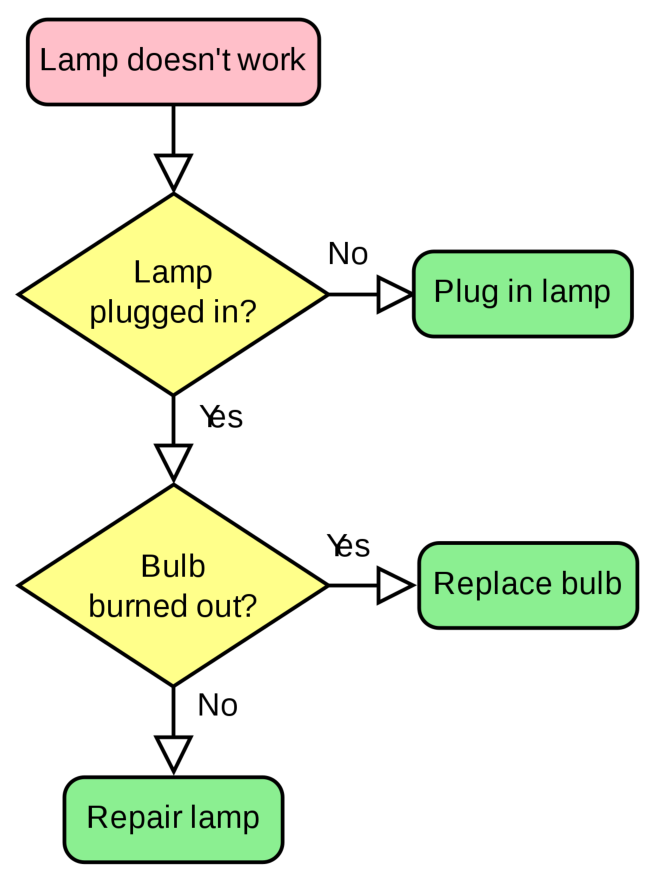
\includegraphics[scale=0.5]{Ch08_Flowchart.pdf}
        \caption{Contoh \textit{Flowchart} (Prosedur Perawatan Lampu)}
        \label{fig:Ch08_Flowchart}
    \end{figure}
    
    Peserta \textit{capstone} harus menyajikan pula model \textit{flowchart} sampai dengan proses pengujian dan verifikasi yang akan digunakan untuk menguji unjuk kerja dari desain yang dibuat. Mahasiswa bisa memilih untuk menggunakan diagram alir, diagram blok, atau algoritme. Salah satu contoh diagram alir dapat dilihat pada Gambar \ref{fig:Ch08_Flowchart}. Program simulasi lain dapat juga berupa program yang digunakan untuk menguji unjuk kerja algoritme yang digunakan untuk menjawab suatu permasalahan. Untuk bidang STL yang tidak menghasilkan perangkat keras maupun program simulasi lengkap, maka peserta \textit{capstone} harus mencantumkan model matematika yang umumnya digunakan. Misalkan, apabila problem yang diangkat berupa problem optimasi, maka peserta \textit{capstone} harus menyertakan \textit{model objective function} serta \textit{constraint} yang berkaitan, dan model algoritme optimasi yang dipakai untuk menyelesaikan problem optimasi berdasarkan sifat dari problem optimasi tersebut (misalkan : \textit{convex}/\textit{non-convex}, linear/\textit{quadratic}/fungsi lainnya, \textit{integer}).


% BAB 09 : Rencana Anggaran dan Jadwal Kegiatan
\chapter{\uppercase{Rencana Anggaran dan Jadwal Kegiatan}}
\label{chap:RAB_JadwalKegiatan}
\textcolor{black}{Di bagian ini, mahasiswa diharapkan mampu mendesain dan mengalokasikan sumber daya (baik berupa manusia, fasilitas, ataupun anggaran keuangan) untuk mendukung solusi yang telah dipilih. Ini dicapai melalui:
\begin{itemize}
    \item kemampuan menguraikan solusi yang dipilih ke dalam sub-tugas (\textit{subtasks}). Hal ini didasarkan pada kenyataan bahwa untuk mencapai solusi akhir, tidak mungkin dilakukan sekali jalan. Hal yang biasa dilakukan adalah solusi akhir dipecah menjadi  beberapa sub-tugas yang dapat ditempuh baik secara serial atau paralel.
    \item pembuatan jadwal kegiatan/\textit{time table} (baik berupa \textit{Gantt chart}, \textit{timeline}, dan sejenisnya) maupun alokasi sumberdaya (seperti manusia, fasilitas, ataupun anggaran keuangan) untuk setiap sub-tugas.
\end{itemize}
Sebagai catatan, alokasi\underline{ sumber daya  manusia dan finansial wajib diberikan}. Alokasi sumber daya manusia mengacu kepada bagaimana tugas atau sub-tugas didistribusikan di antara anggota kelompok, sedangkan alokasi finansial mengacu kepada alokasi biaya yang dibutuhkan untuk menjalankan proyek. Alokasi biaya tidak harus berupa biaya yang benar-benar dikeluarkan mahasiswa. Sebagai contoh jika salah satu yang diperlukan dari solusi anda adalah sebuah sensor yang berharga 100.000.000 rupiah dan anda mendapatkan pinjaman sensor tersebut dari salah satu lab di DTETI, maka anda harus memasukkan harga sensor tersebut ke dalam alokasi biaya anda.
}


Pada bagian ini, tuliskan komponen biaya yang mungkin timbul dari pelaksanaan kegiatan \textit{Capstone}. Komponen biaya terdiri dari biaya operasional, seperti pembelian barang/bahan penelitian, biaya pengujian/analisis, penyewaan peralatan, dan penyelenggaraan workshop/pelatihan/\textit{survey}. Komponen biaya mencakup semua biaya yang dikeluarkan oleh semua pihak, baik dari pihak mahasiswa, dosen pembimbing, maupun institusi. Dalam konteks \textit{Capstone}, dimungkinkan komponen biaya bernilai nol, misalnya bila hanya dibutuhkan peralatan berupa laptop yang telah lazim dimiliki setiap individu. Selain rencana anggaran, rencana pelaksanaan kegiatan juga perlu disajikan pada bagian ini. Tuliskan rencana kegiatan mulai dari bulan Agustus 2021 sampai dengan bulan Juli 2022.

\section{Rencana Anggaran Pelaksanaan \textit{Capstone}}

    Bagian ini berisi estimasi biaya yang diperlukan untuk pembelian bahan dan peralatan dalam pelaksanaan kegiatan \textit{Capstone}. Tabel \ref{tab:estimasi_anggaran} merupakan contoh tabel yang berisi estimasi biaya yang diperlukan untuk pelaksanaan kegiatan \textit{Capstone}. Bila bahan atau peralatan sudah tersedia di laboratorium (Lab.), mahasiswa hanya perlu menambahkan penjelasan bahwa bahan dan peralatan sudah tersedia di laboratorium dan tidak perlu menuliskannya di dalam tabel.

        \begin{longtable}{|clcc|c|}
            \caption{Estimasi Anggaran Pelaksanaan Kegiatan \textit{Capstone}}
            \label{tab:estimasi_anggaran}
            \vspace{-0.75em}\\
            \hline
\multicolumn{1}{|c|}{\textbf{No.}} & \multicolumn{1}{c|}{\textbf{Barang}} & \multicolumn{1}{c|}{\textbf{Jumlah}} & \textbf{Harga Satuan} & \textbf{Total Harga} \\ 
            \hline
\multicolumn{1}{|c|}{1}            & \multicolumn{1}{l|}{Lampu LED}       & \multicolumn{1}{c|}{4}               & Rp 47.500,00          & Rp 190.000,00        \\ 
            \hline
\multicolumn{1}{|c|}{2}            & \multicolumn{1}{l|}{Modul Sensor IR} & \multicolumn{1}{c|}{1}               & Rp 28.500,00          & Rp 28.500,00         \\ 
            \hline
\multicolumn{4}{|c|}{\textbf{TOTAL}}                                                                                                     & Rp xxx.xxx,xx        \\ 
            \hline
        \end{longtable}
        
\section{Jadwal Pelaksanaan Kegiatan \textit{Capstone}}

    Berikan \textit{overview} tentang target waktu pelaksanaan proyek akhir ini. Tabel \ref{tab:jadwal_pelaksanaan} di bawah ini merupakan contoh tentang pelaksanaan tugas akhir yang diselesaikan dalam waktu 6 bulan. Pastikan keselarasan jadwal dengan prosedur pelaksanaan. \textbf{Tim mahasiswa wajib menggunakan standard Gantt Chart.}
    
        \begin{longtable}{|l|cccccccccccc|}
            \caption{Jadwal Pelaksanaan Kegiatan \textit{Capstone}}
            \label{tab:jadwal_pelaksanaan}
            \vspace{-0.75em}\\
            \hline
\multicolumn{1}{|c|}{}                                 & \multicolumn{12}{c|}{Bulan ke-}                                                                                                                                                                                                                                                                                                                                                                                                                                                                                                                                          \\ \cline{2-13} 
\multicolumn{1}{|c|}{\multirow{-2}{*}{Tahap Kegiatan}} & \multicolumn{1}{c|}{1}                        & \multicolumn{1}{c|}{2}                        & \multicolumn{1}{c|}{3}                        & \multicolumn{1}{c|}{4}                        & \multicolumn{1}{c|}{5}                        & \multicolumn{1}{c|}{6}                        & \multicolumn{1}{c|}{7}                        & \multicolumn{1}{c|}{8}                        & \multicolumn{1}{c|}{9}                        & \multicolumn{1}{c|}{10}                       & \multicolumn{1}{c|}{11}                       & 12                       \\ \hline
\textbf{Persiapan}                                              & \multicolumn{1}{c|}{}                         & \multicolumn{1}{c|}{}                         & \multicolumn{1}{c|}{}                         & \multicolumn{1}{c|}{}                         & \multicolumn{1}{c|}{}                         & \multicolumn{1}{c|}{}                         & \multicolumn{1}{c|}{}                         & \multicolumn{1}{c|}{}                         & \multicolumn{1}{c|}{}                         & \multicolumn{1}{c|}{}                         & \multicolumn{1}{c|}{}                         &                          \\
a. Studi Literatur                                     & \multicolumn{1}{c|}{\cellcolor[HTML]{333333}} & \multicolumn{1}{c|}{\cellcolor[HTML]{333333}} & \multicolumn{1}{c|}{}                         & \multicolumn{1}{c|}{}                         & \multicolumn{1}{c|}{}                         & \multicolumn{1}{c|}{}                         & \multicolumn{1}{c|}{}                         & \multicolumn{1}{c|}{}                         & \multicolumn{1}{c|}{}                         & \multicolumn{1}{c|}{}                         & \multicolumn{1}{c|}{}                         &                          \\
b. Desain                                              & \multicolumn{1}{c|}{}                         & \multicolumn{1}{c|}{}                         & \multicolumn{1}{c|}{\cellcolor[HTML]{333333}} & \multicolumn{1}{c|}{\cellcolor[HTML]{333333}} & \multicolumn{1}{c|}{}                         & \multicolumn{1}{c|}{}                         & \multicolumn{1}{c|}{}                         & \multicolumn{1}{c|}{}                         & \multicolumn{1}{c|}{}                         & \multicolumn{1}{c|}{}                         & \multicolumn{1}{c|}{}                         &                          \\
c. Pembelian Bahan                                     & \multicolumn{1}{c|}{}                         & \multicolumn{1}{c|}{}                         & \multicolumn{1}{c|}{}                         & \multicolumn{1}{c|}{\cellcolor[HTML]{333333}} & \multicolumn{1}{c|}{\cellcolor[HTML]{333333}} & \multicolumn{1}{c|}{}                         & \multicolumn{1}{c|}{}                         & \multicolumn{1}{c|}{}                         & \multicolumn{1}{c|}{}                         & \multicolumn{1}{c|}{}                         & \multicolumn{1}{c|}{}                         &                          \\
\textbf{Pelaksanaan}                                            & \multicolumn{1}{c|}{}                         & \multicolumn{1}{c|}{}                         & \multicolumn{1}{c|}{}                         & \multicolumn{1}{c|}{}                         & \multicolumn{1}{c|}{}                         & \multicolumn{1}{c|}{}                         & \multicolumn{1}{c|}{}                         & \multicolumn{1}{c|}{}                         & \multicolumn{1}{c|}{}                         & \multicolumn{1}{c|}{}                         & \multicolumn{1}{c|}{}                         &                          \\
a. Pembuatan Prototipe                                 & \multicolumn{1}{c|}{}                         & \multicolumn{1}{c|}{}                         & \multicolumn{1}{c|}{}                         & \multicolumn{1}{c|}{}                         & \multicolumn{1}{c|}{}                         & \multicolumn{1}{c|}{\cellcolor[HTML]{333333}} & \multicolumn{1}{c|}{\cellcolor[HTML]{333333}} & \multicolumn{1}{c|}{}                         & \multicolumn{1}{c|}{}                         & \multicolumn{1}{c|}{}                         & \multicolumn{1}{c|}{}                         &                          \\
b. Pengujian Kinerja                                   & \multicolumn{1}{c|}{}                         & \multicolumn{1}{c|}{}                         & \multicolumn{1}{c|}{}                         & \multicolumn{1}{c|}{}                         & \multicolumn{1}{c|}{}                         & \multicolumn{1}{c|}{}                         & \multicolumn{1}{c|}{\cellcolor[HTML]{333333}} & \multicolumn{1}{c|}{\cellcolor[HTML]{333333}} & \multicolumn{1}{c|}{}                         & \multicolumn{1}{c|}{}                         & \multicolumn{1}{c|}{}                         &                          \\
c. Evaluasi dan Perbaikan                              & \multicolumn{1}{c|}{}                         & \multicolumn{1}{c|}{}                         & \multicolumn{1}{c|}{}                         & \multicolumn{1}{c|}{}                         & \multicolumn{1}{c|}{}                         & \multicolumn{1}{c|}{}                         & \multicolumn{1}{c|}{\cellcolor[HTML]{333333}} & \multicolumn{1}{c|}{\cellcolor[HTML]{333333}} & \multicolumn{1}{c|}{\cellcolor[HTML]{333333}} & \multicolumn{1}{c|}{\cellcolor[HTML]{333333}} & \multicolumn{1}{c|}{\cellcolor[HTML]{333333}} &                          \\
\textbf{Penyelesaian}                                           & \multicolumn{1}{c|}{}                         & \multicolumn{1}{c|}{}                         & \multicolumn{1}{c|}{}                         & \multicolumn{1}{c|}{}                         & \multicolumn{1}{c|}{}                         & \multicolumn{1}{c|}{}                         & \multicolumn{1}{c|}{}                         & \multicolumn{1}{c|}{}                         & \multicolumn{1}{c|}{}                         & \multicolumn{1}{c|}{}                         & \multicolumn{1}{c|}{}                         &                          \\
a. \textit{Finishing}                                           & \multicolumn{1}{c|}{}                         & \multicolumn{1}{c|}{}                         & \multicolumn{1}{c|}{}                         & \multicolumn{1}{c|}{}                         & \multicolumn{1}{c|}{}                         & \multicolumn{1}{c|}{}                         & \multicolumn{1}{c|}{}                         & \multicolumn{1}{c|}{}                         & \multicolumn{1}{c|}{}                         & \multicolumn{1}{c|}{\cellcolor[HTML]{333333}} & \multicolumn{1}{c|}{\cellcolor[HTML]{333333}} &                          \\
b. Pembuatan Laporan                                   & \multicolumn{1}{c|}{}                         & \multicolumn{1}{c|}{}                         & \multicolumn{1}{c|}{}                         & \multicolumn{1}{c|}{}                         & \multicolumn{1}{c|}{}                         & \multicolumn{1}{c|}{}                         & \multicolumn{1}{c|}{}                         & \multicolumn{1}{c|}{}                         & \multicolumn{1}{c|}{}                         & \multicolumn{1}{c|}{}                         & \multicolumn{1}{c|}{\cellcolor[HTML]{333333}} & \cellcolor[HTML]{333333} \\ \hline

        \end{longtable}

% BAB 10 : Simulasi Pendahuluan 
\chapter{\uppercase{Simulasi Pendahuluan}}
\label{chap:Simulasi_Pendahuluan}
Pada bagian ini, apabila diperlukan Anda dapat menyertakan simulasi pengantar. Simulasi pengantar ini tidak harus berupa program simulasi. Sebagai contoh dalam perancangan perangkat keras, peserta dapat menyampaikan simulasi perangkat keras yang di desain dengan menggunakan perangkat lunak bawaan (\textit{tools}) misalkan Orchad/PSpice untuk mensimulasikan bagian-bagian dari keseluruhan desain misalnya jika desain berupa perangkat keras lengkap dimana bagian-bagian perangkat keras tersebut terdapat \textit{low-pass filter}, \textit{high-pass filter}, ADC (\textit{Analog-to-Digital Converter}), dan DAC (\textit{Digital-to-Analog Converter}), maka Anda perlu mensimulasikan komponen-komponen \textit{low-pass filter},\textit{ high-pass filter,} ADC, dan DAC sesuai dengan desain yang diinginkan. Misalnya peserta akan mendesain \textit{low-pass filter} Butterworth dengan frekuensi \textit{cut-off} 100 Hz, maka peserta perlu merancang komponen $R$ dan $C$ serta mensimulasikan dengan perangkat lunak yang tersedia.

Jika mensimulasikan operasi sistem tenaga listrik, peserta bisa menggunakan perangkat lunak yang biasa dipakai misalkan Digsilent, ETAP dan lain-lain. Jika model yang dihasilkan berupa \textit{model multi machines} yang terinterkoneksi dengan beban, maka Anda dapat mendesain simulasi berdasarkan perangkat lunak (misalnya MATLAB) menjadi bagian-bagian kecil dari sistem tersebut. Anda bisa mensimulasikan satu generator yang dipakai jika disambungkan ke \textit{infinite bus}, selain itu bisa mensimulasikan saluran transmisi, mensimulasikan beban-beban aktif dan reaktif, mensimulasikan motor, mensimulasikan PV, dan sebagainya.


% BAB 11 : Kesimpulan 
\chapter{\uppercase{Kesimpulan}}
\label{chap:Kesimpulan}
Kesimpulan pada dokumen C-251 ini berupa ringkasan dari proses desain produk, program, atau perangkat lunak yang akan dibuat, beserta rencana bagaimana desain ini akan diimplementasikan.

% ------------------------------------------------------------ %
% References

\begin{thebibliography}{}

    \bibitem{edwards_sliding_1998}
Edwards,~C. and Spurgeon,~S.~K., \emph{Sliding Mode Control: Theory and Applications}, London, UK, 1998

\bibitem{b1} 
G. Eason, B. Noble, and I. N. Sneddon, ``On certain integrals of Lipschitz-Hankel type involving products of Bessel functions,'' Phil. Trans. Roy. Soc. London, vol. A247, pp. 529--551, April 1955.

\bibitem{b2} 
J. Clerk Maxwell, A Treatise on Electricity and Magnetism, 3rd ed., vol. 2. Oxford: Clarendon, 1892, pp.68--73.

\bibitem{b3} 
I. S. Jacobs and C. P. Bean, ``Fine particles, thin films and exchange anisotropy,'' in Magnetism, vol. III, G. T. Rado and H. Suhl, Eds. New York: Academic, 1963, pp. 271--350.

\end{thebibliography}

% Akhir Dokumen
\end{document}